\documentclass[]{article}
\usepackage{lmodern}
\usepackage{amssymb,amsmath}
\usepackage{ifxetex,ifluatex}
\usepackage{fixltx2e} % provides \textsubscript
\ifnum 0\ifxetex 1\fi\ifluatex 1\fi=0 % if pdftex
  \usepackage[T1]{fontenc}
  \usepackage[utf8]{inputenc}
\else % if luatex or xelatex
  \ifxetex
    \usepackage{mathspec}
  \else
    \usepackage{fontspec}
  \fi
  \defaultfontfeatures{Ligatures=TeX,Scale=MatchLowercase}
\fi
% use upquote if available, for straight quotes in verbatim environments
\IfFileExists{upquote.sty}{\usepackage{upquote}}{}
% use microtype if available
\IfFileExists{microtype.sty}{%
\usepackage{microtype}
\UseMicrotypeSet[protrusion]{basicmath} % disable protrusion for tt fonts
}{}
\usepackage[margin=1in]{geometry}
\usepackage{hyperref}
\hypersetup{unicode=true,
            pdfborder={0 0 0},
            breaklinks=true}
\urlstyle{same}  % don't use monospace font for urls
\usepackage{graphicx,grffile}
\makeatletter
\def\maxwidth{\ifdim\Gin@nat@width>\linewidth\linewidth\else\Gin@nat@width\fi}
\def\maxheight{\ifdim\Gin@nat@height>\textheight\textheight\else\Gin@nat@height\fi}
\makeatother
% Scale images if necessary, so that they will not overflow the page
% margins by default, and it is still possible to overwrite the defaults
% using explicit options in \includegraphics[width, height, ...]{}
\setkeys{Gin}{width=\maxwidth,height=\maxheight,keepaspectratio}
\IfFileExists{parskip.sty}{%
\usepackage{parskip}
}{% else
\setlength{\parindent}{0pt}
\setlength{\parskip}{6pt plus 2pt minus 1pt}
}
\setlength{\emergencystretch}{3em}  % prevent overfull lines
\providecommand{\tightlist}{%
  \setlength{\itemsep}{0pt}\setlength{\parskip}{0pt}}
\setcounter{secnumdepth}{0}
% Redefines (sub)paragraphs to behave more like sections
\ifx\paragraph\undefined\else
\let\oldparagraph\paragraph
\renewcommand{\paragraph}[1]{\oldparagraph{#1}\mbox{}}
\fi
\ifx\subparagraph\undefined\else
\let\oldsubparagraph\subparagraph
\renewcommand{\subparagraph}[1]{\oldsubparagraph{#1}\mbox{}}
\fi

%%% Use protect on footnotes to avoid problems with footnotes in titles
\let\rmarkdownfootnote\footnote%
\def\footnote{\protect\rmarkdownfootnote}

%%% Change title format to be more compact
\usepackage{titling}

% Create subtitle command for use in maketitle
\newcommand{\subtitle}[1]{
  \posttitle{
    \begin{center}\large#1\end{center}
    }
}

\setlength{\droptitle}{-2em}
  \title{}
  \pretitle{\vspace{\droptitle}}
  \posttitle{}
  \author{}
  \preauthor{}\postauthor{}
  \date{}
  \predate{}\postdate{}

\usepackage{float} \usepackage{hyperref} \usepackage{gensymb}

\begin{document}

2017 \vspace{4cm}

\begin{center}
{\Large Why most studied populations should decline}

\vspace{4cm}

\end{center}

\section{Methods: Portal data analysis}

To test the site selection hypothesis, a time series with plot
replicates was needed. However, in most ecological monitoring, there is
a trade-off in sampling spatially or temporally. Typically, a long time
series consists of a single population. We wanted to investigate the
effect of biased sampling and therefore needed a long time series with
multiple plot replicates.

We examined data from the Portal Project. The project consists of
long-term monitoring of a Chihuahuan Desert ecosystem near Portal,
Arizona, USA (Ernest et al. 2009). Since 1978, 24 individual replicate
plots have been sampled. Monitoring includes ants, plants, and rodents.
The experimental design, with replicates of plots, allows us to test
ideas of sampling bias. Thus, we explored biased subsets of the data and
observed the effect of the sampling on assessing long-term trends.

We compared two subsets of data: 1) total abundance of the two initially
(in the first year) most abundant plots and 2) random selections of any
pair of plots. This biased sampling allowed us to see the effect of only
sampling the most common plots. We then used simple linear regression to
estimate the population increase or decrease over time. We hypothesized
that the initially most abundant plots should see significantly larger
declines (i.e.~more negative slope estimates) than the random subsets of
plots.

We also examined the effect of removing the first five years of data. We
hypothesized that by removing the first five years, that we should
reduce bias in selecting only the most common sites.

\section{Results: Portal data}

\begin{figure}
\centering
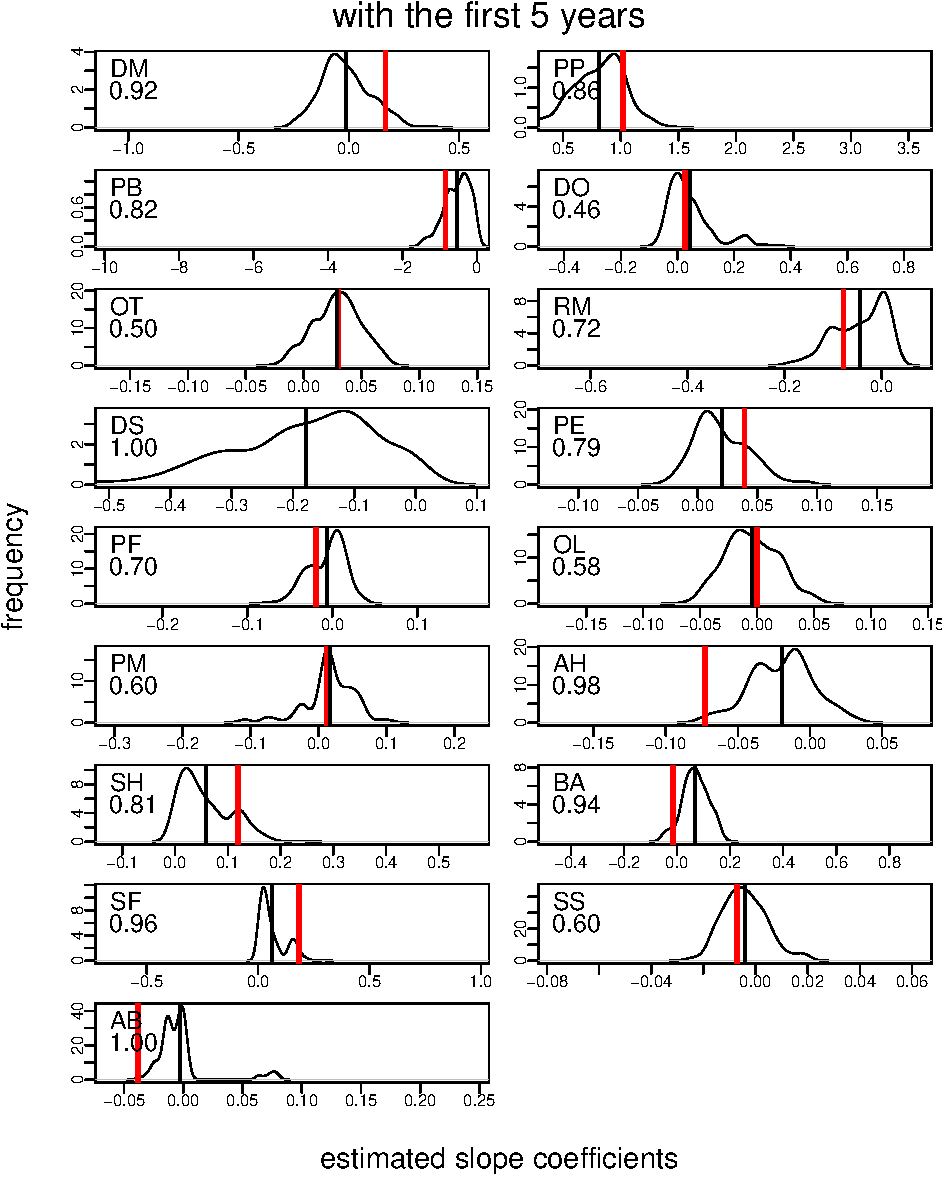
\includegraphics{Empirical_Investigation_files/figure-latex/unnamed-chunk-2-1.pdf}
\caption{This figure denotes the subset of data where the first five
years of data are included. Each plot represents a single species. Each
plot has a distribution of slope values for random pairs of sites over
time. THe vertical black line is the mean of this distirbution. The
vertical, red line denotes the estimated slope for the two most abundant
sites over time. The number in the top-right of the plot is the fraction
of the distribution less than or greater than the slope estimate for the
most common sites.\label{fig:common_vs_random_with5}}
\end{figure}

\begin{figure}
\centering
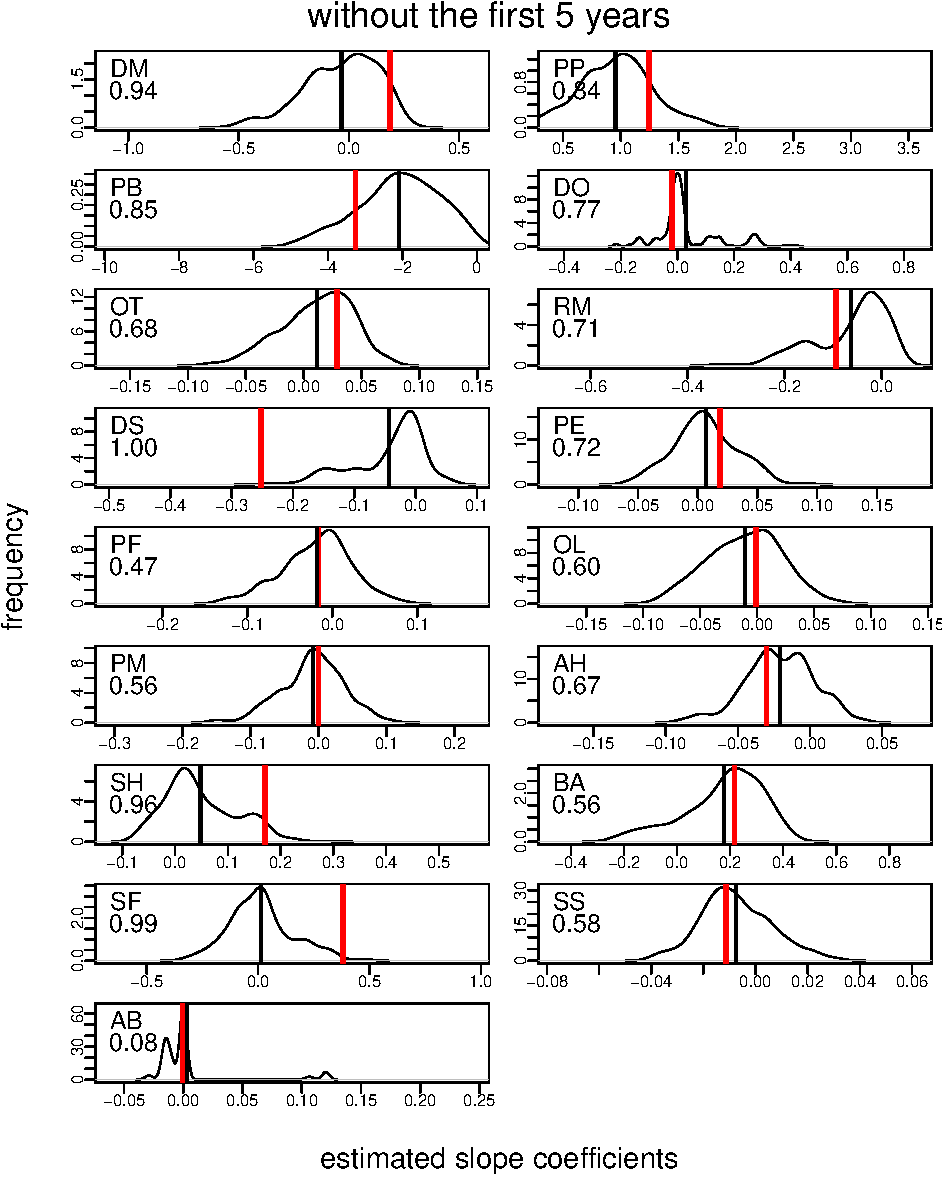
\includegraphics{Empirical_Investigation_files/figure-latex/unnamed-chunk-3-1.pdf}
\caption{This figure denotes the subset of data where the first five
years of data are not included. Each plot represents a single species.
Each plot has a distribution of slope values for random pairs of sites
over time. THe vertical black line is the mean of this distirbution. The
vertical, red line denotes the estimated slope for the two most abundant
sites over time. The number in the top-right of the plot is the fraction
of the distribution less than or greater than the slope estimate for the
most common sites.\label{fig:common_vs_random_without5}}
\end{figure}

We compared the predicted slope from linear regression for the two most
common plots versus pairs of random plots. We found that the most common
plots differ from pairs of random plots (Fig.
\ref{fig:common_vs_random_with5}). For XX out of the XX species, the
slope from the most common plots were significantly different than
choosing plots at random. For XX cases (except XX) where the most common
plots had a significantly different slope, the most common plots had a
slope coefficient much more negative than random plot slopes.

We then removed the first five years of data. We hypothesized that this
would help ameliorate some of the effect of choosing to sample only the
most common plots. We found that fewer slopes from the common plots were
statistically different from random slopes, although the effects still
persisted (Fig. \ref{fig:common_vs_random_without5}).

Alternatively, we can also just examine the species with observed
declines over time. In Fig. \ref{fig:declining_species} we examine the
effect of removing the first five years of data for only these declining
species. We see that removing the first five years of data either had no
effect, or slightly reduced the difference between choosing random plots
and choosing the most common plots (Fig. \ref{fig:declining_species}).

\begin{figure}
\centering
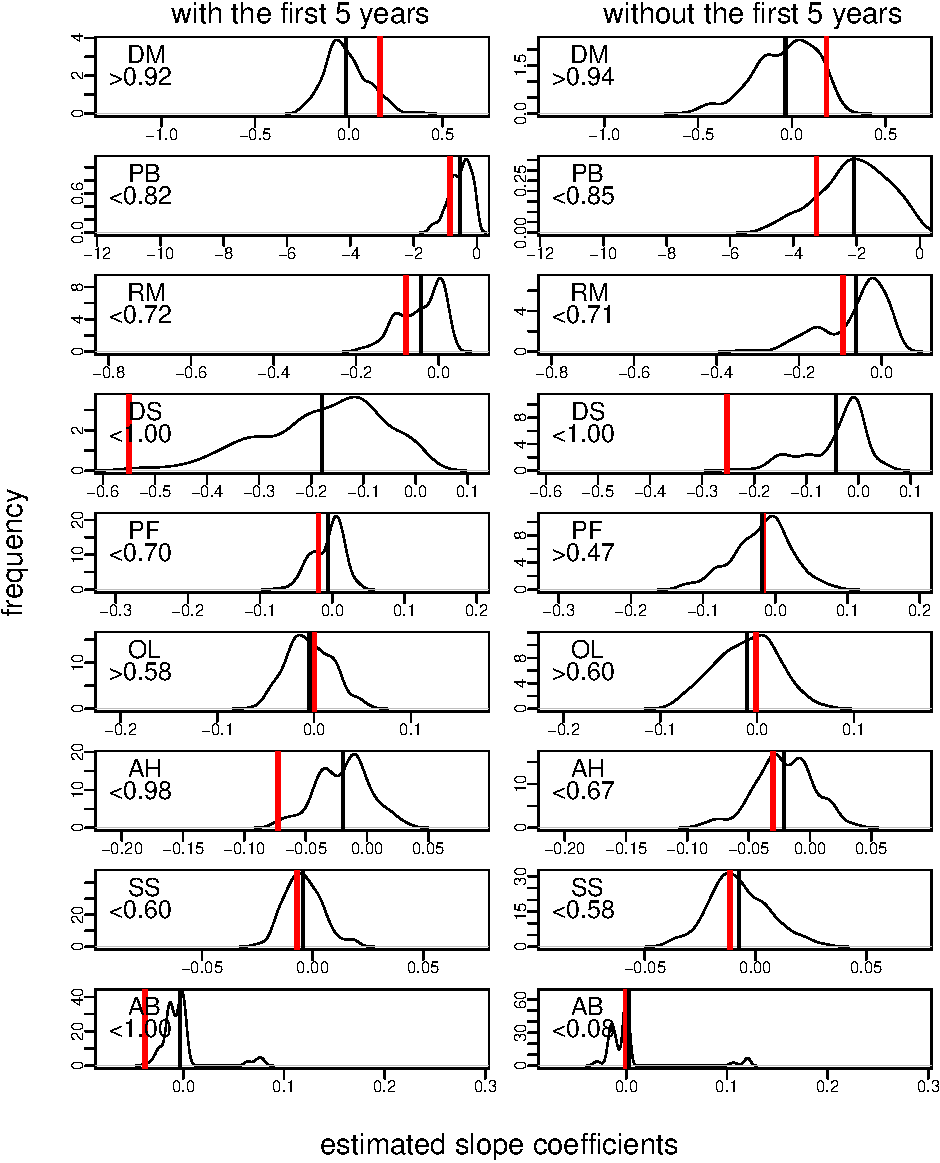
\includegraphics{Empirical_Investigation_files/figure-latex/unnamed-chunk-4-1.pdf}
\caption{This figure denotes the subset of time series where the trend
in population size was declining. Each row represents a single species.
Each plot has a distribution of slope values for random pairs of sites
over time. The vertical black line is the mean of this distirbution. The
vertical, red line denotes the estimated slope for the two most abundant
sites over time. The number in the top-right of the plot is the fraction
of the distribution less than or greater than the slope estimate for the
most common sites.\label{fig:declining_species}}
\end{figure}

\pagebreak

\section{Methods: GPDD exploration}

We also examined time series data from different sources incuding the
Global Population Dynamics Database, compiled by @Keith2015. This data
does not have replicate plots like the Portal data. Instead, the
database consists of time series for individual populations. We wanted
to see the effect of two different forms of bias sampling. First,

We wanted to see the effect of sampling a population starting at a high
point. The rational being that when initiating a survey you may start
with a population at high abundance for logistical reasons.

We selected only time series with 40+ years of data to ensure high
statistical power (White 2017). Then, for each population time series we
examined two subsets of data: 1) sampling for 15 years starting at the
time series high point, and 2) sampling for seven years on either side
of the time series high point. The latter subset is to represent a
situation where you remove some of the bias associated with only
sampling populations at high abundance.

\section{Results: GPDD exploration}

\begin{figure}
\centering
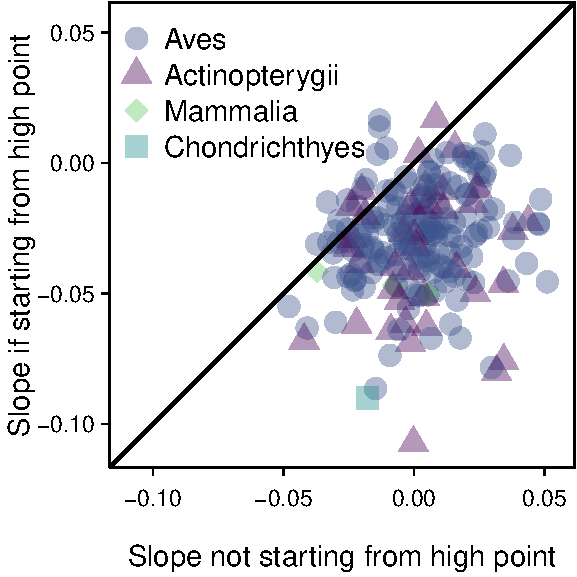
\includegraphics{Empirical_Investigation_files/figure-latex/unnamed-chunk-5-1.pdf}
\caption{Slope estimate from linear regression for biased sample of
starting at the high point in the time series versus not sampling at the
high point. Any points below the identity line are situations where the
slope estimate starting from the high point was less than that of
sampling not starting from the high point.\label{fig:GPDD_high_point}}
\end{figure}

We explored time series data for 202 populations of mammals, fish, and
birds. For each time series, we examined two different subsets: either
starting at the time series high point or not. As we hypothesized, the
slope of a time series starting from a high point was typically more
negative than situations not sampled starting from a high point (Fig.
\ref{fig:GPDD_high_point}).

Potential explanatory variables (e.g.~class, variance in population
size, autocorrelation generation size) did not strongly predict which
time series were more likely to be affected by biased sampling of high
populations (Fig. \ref{fig:GPDD_explanatory}).

\begin{figure}
\centering
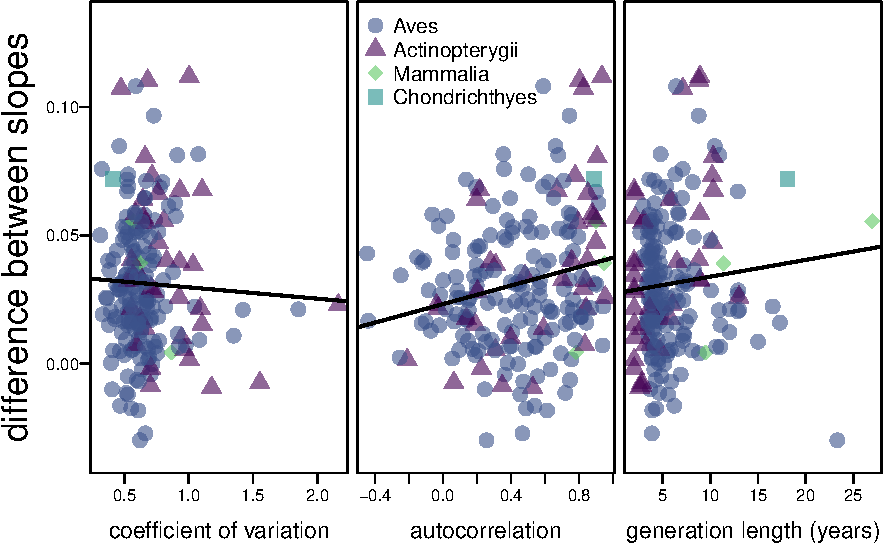
\includegraphics{Empirical_Investigation_files/figure-latex/unnamed-chunk-6-1.pdf}
\caption{Slope estimate from linear regression for biased sample of
starting to sample at the high point in the time series versus not
sampling at the high point. Any points below the identity line are
situations where the slope estimate starting from the high point was
less than that of sampling not starting from the high
point.\label{fig:GPDD_explanatory}}
\end{figure}

\pagebreak

\section{Removing initial years of time series}

\begin{figure}
\centering
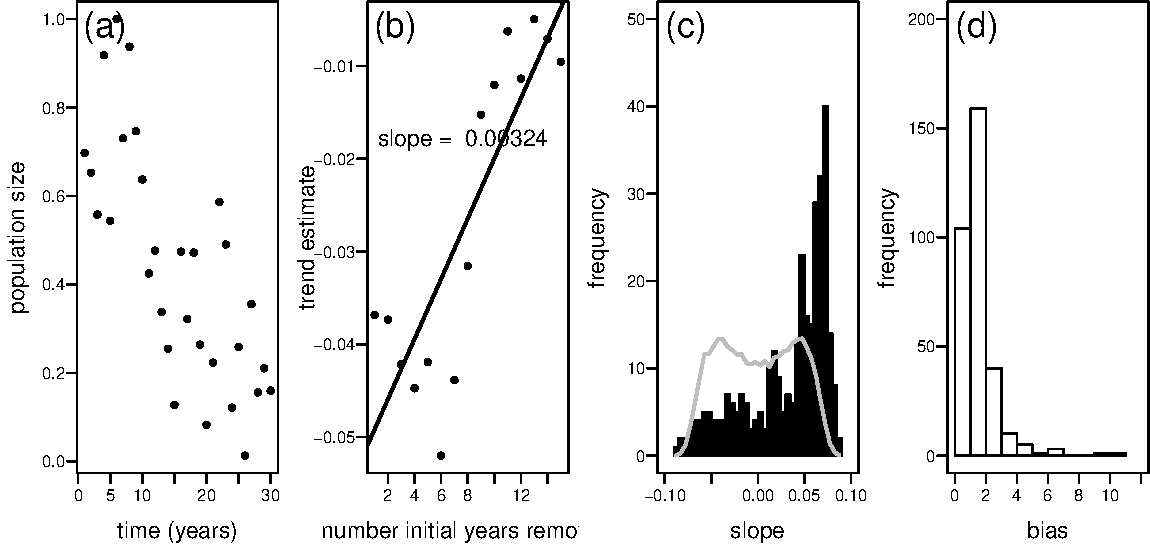
\includegraphics{Empirical_Investigation_files/figure-latex/unnamed-chunk-8-1.pdf}
\caption{(a) Example time series from the Global Population Dynamics
Database. (b) The trend in population size (i.e.~the estimated slope
coefficient) for different numbers of initial years removed from the
data. In other words, we estimate the trend in abundance from years 1
through 15, then 2 through 16, and so forth. (c) Frequency of the slopes
estimated to fit data in (b) for each species (n = 358). A positive
value indicates the estimated trend in abundance over time becomes less
negative when you remove more initial years. The dark line is the null
distribution generated using simulated data. (d) The degree to which
removing initial years affects the trend estimates. For example, A bias
of 2.5 would indicate that not removing the first 10 years of data
increases the estimated slope by 2.5 times.
\label{fig:removing_initial_years}}
\end{figure}

We also examined the effect of removing years from the beginning of the
time series. The rationale here being that a census may have started in
a year when a species was at a particularly high abundance. Therefore,
the time series would start off artificially high. We subsampled each
time series to remove initial years from the data. In other words, we
examine the population size in years 1 through 15, then years 2 through
15, and so forth. We then examined how the estimated change in abundance
(the slope coefficient) changed with more initial years removed. An
example of this is shown in figure \ref{fig:removing_initial_years}b.
Here, a positive relationship between the trend estimate (slope
coefficient) and number of initial years removed would indicate a
situation where the initial years of the time series did in fact cause
the abundance trends to be more negative.

We then examined the estimated relationship between trend estimate and
the number of initial years removed for each declining species (Fig.
\ref{fig:removing_initial_years}c). Here, a positive value for slope
would indicate that the initial years of a time series were artificially
high and these caused larger estimated declines. We see that there is a
large number of time series with slope values between 0.05 and 0.1 (Fig.
\ref{fig:removing_initial_years}c). The dark line is a null expectation
of this data. To obtain this null distribution, we simulated time series
where the initial years were not biased to be larger values.


\end{document}
